\documentclass[runningheads]{llncs}
%
\renewcommand{\figurename}{Figure}

\usepackage[T1]{fontenc}
\usepackage{graphicx}
\usepackage{amsmath}
\usepackage{amssymb}
\usepackage{float}
\usepackage{multirow}
\usepackage{booktabs}
\usepackage{marvosym}
\usepackage{ifsym}
\usepackage[table]{xcolor}
\usepackage{placeins}
\usepackage[autostyle=false, style=english]{csquotes}\MakeOuterQuote{"}

% hyperref must be loaded last; makes \cite, \ref and URLs clickable
\usepackage{hyperref}
\hypersetup{
  colorlinks=true,
  linkcolor={blue!55!black},
  citecolor={blue!55!black},
  urlcolor={blue!55!black}
}

\renewcommand{\arraystretch}{1.2}

\graphicspath{{figures/}}

\definecolor{best}{HTML}{1A4DAB}
\newcommand{\best}[1]{\textcolor{best}{\textbf{#1}}}

\begin{document}
%
\title{A Frozen BiomedCLIP Branch as a Cross-Dataset Regularizer for Imbalanced Lumbar Disc Grading and Zero-Shot Label-Space Extension}
%
\titlerunning{BiomedCLIP Regularizer for Lumbar Disc Grading}
%
% ----- DOUBLE-BLIND submission (MIWAI 2026): authors anonymized -----
% Camera-ready author block (uncomment for final version):
% \author{Trung Kien Ha\inst{1,2} \and
% Trong Nhan Phan\inst{1,2}\textsuperscript{\Letter}}
% \authorrunning{T. K. Ha and T. N. Phan}
% \institute{Faculty of Computer Science and Engineering, Ho Chi Minh City University of Technology (HCMUT), 268 Ly Thuong Kiet, District 10, Ho Chi Minh City, Vietnam.\\
% \and Vietnam National University Ho Chi Minh City (VNU-HCM), Linh Trung Ward, Thu Duc City, Ho Chi Minh City, Vietnam.\\
% \email{htkien.sdh242@hcmut.edu.vn, nhanpt@hcmut.edu.vn}}
%
\author{Anonymous Author(s)}
\authorrunning{Anonymous}
\institute{Affiliation withheld for double-blind review}
%
\maketitle
%
\begin{abstract}
Automated grading of lumbar intervertebral disc (IVD) pathology on MRI is clinically useful but hard: severity classes are heavily imbalanced and large labelled volumetric corpora are scarce. We present a two-branch hybrid model that fuses a 3D ResNet-34 with Convolutional Block Attention Modules (CBAM) and a frozen BiomedCLIP image-text encoder, trained on the RSNA 2024 Lumbar Degenerative Classification dataset. The CBAM-3D branch captures cross-slice anatomical context, while the BiomedCLIP branch supplies a semantic prior from large-scale biomedical pretraining; a small trainable concat-MLP merges the two streams into a text-aligned embedding for both supervised classification and zero-shot label-space extension. With focal loss, square-root class weights, minority oversampling, and SpineNetV2-style augmentation, across three seeds the hybrid lifts Severe-class recall from 12.3\% to 48.6\%, Severe F1 from 0.152 to 0.356, and Severe AUC from 0.872 to 0.899. Without any SPIDER fine-tuning, the same model extends zero-shot to eight unseen SPIDER labels via text prompts (mean F1 = 0.362), with gains concentrated on disc-morphology labels semantically close to the training schema. Under three-seed supervised transfer the hybrid matches SpineNetV2 on aggregate SPIDER F1 ($0.653$ vs.\ $0.646$) and exceeds the CBAM-only variant ($0.619$) by $+0.034$ (paired $t$-test over three seeds, $p=0.011$); we interpret this behavioral pattern as the frozen BiomedCLIP branch acting as a cross-dataset regularizer that offsets CBAM's tendency to overfit RSNA-specific patterns.

\keywords{spine MRI \and intervertebral disc grading \and attention \and vision-language models \and BiomedCLIP \and zero-shot classification \and class imbalance.}
\end{abstract}
%
%==============================================%
\section{Introduction}\label{sec1}

Low back pain is the leading cause of disability worldwide, and lumbar disc degeneration drives most of the surgical and conservative interventions that follow. Quantitative MRI grading of intervertebral disc (IVD) pathology, including spinal canal stenosis, left and right neural foraminal stenosis, and Pfirrmann grade, is still done largely by hand and carries substantial inter-rater variability~\cite{nigru2024}.

Automated systems built on 3D convolutional networks such as SpineNet~\cite{jamaludin2017} and SpineNetV2~\cite{windsor2022} have made real progress, yet two problems remain open. The first is class imbalance. Clinically, the most important class (Severe) is usually fewer than 5\% of the training samples, and ordinary cross-entropy training produces models that ignore the minority class almost completely, with Severe recall close to zero. The second is a fixed label space. A model trained on one labelling schema, for example the 3-condition $\times$ 3-severity grid of RSNA 2024, cannot answer a query phrased in another schema, such as the Pfirrmann, spondylolisthesis, and herniation labels of SPIDER, without retraining a new fixed-class head.

We tackle both problems with a single hybrid model. Our main contributions, centered on the cross-dataset transfer finding, are as follows.
\begin{itemize}
    \item A \textbf{cross-dataset regularization finding}. In a three-seed SPIDER transfer experiment, adding CBAM to the ResNet-34 backbone lowers aggregate F1 by $0.027$ (beyond the pooled seed standard deviation), indicating that the attention module that helps in-domain RSNA Severe metrics hurts cross-center generalization. The proposed hybrid (CBAM with frozen BiomedCLIP) recovers above the CBAM-only configuration by $+0.034$ (paired $t$-test over three seeds, $p=0.011$), a behavioral pattern consistent with the BiomedCLIP branch acting as a regularizer.
    \item A \textbf{two-branch hybrid architecture} that combines a CBAM-3D ResNet-34~\cite{woo2018cbam,he2016resnet} with a frozen BiomedCLIP~\cite{zhang2023biomedclip} encoder and a learned concat-MLP fusion head. The ablation confirms that the two branches contribute along complementary axes: in-domain Severe metrics versus cross-center robustness.
    \item A \textbf{cross-dataset label-space extension}. By routing the fused embedding through cosine similarity against text-prompt embeddings, the same RSNA-trained model transfers to the eight unseen SPIDER labels with no SPIDER fine-tuning, reaching mean F1 = 0.362 zero-shot. With lightweight supervised transfer over three seeds, the hybrid leads on rare-class recall, for example Disc Herniation Yes ($0.36 \pm 0.08$ vs.\ $0$ for both SpineNetV2 and CBAM).
    \item A \textbf{class-imbalance training pipeline} (focal loss~\cite{lin2017focal}, square-root class weights, minority oversampling, and medical augmentation) that raises Severe-class recall from 12.3\% to 48.6\% (three-seed mean) on RSNA 2024.
\end{itemize}

To our knowledge, no prior peer-reviewed work has applied BiomedCLIP to RSNA 2024 lumbar classification, and none has reported a zero-shot label-space extension on the same architecture for lumbar spine MRI.

The rest of the paper is organized as follows. Section~\ref{sec2} reviews related work. Section~\ref{sec3} describes the proposed architecture and training workflow. Section~\ref{sec4} reports experiments and analysis on RSNA 2024 and SPIDER. Section~\ref{sec5} concludes the paper.

%==============================================%
\section{Related Work}\label{sec2}

\textbf{Lumbar disc grading.}
Jamaludin et al.~\cite{jamaludin2017} introduced SpineNet, a VGG-style 2D CNN trained on the GENODISC corpus. Windsor et al.~\cite{windsor2022} upgraded the backbone to a 3D ResNet-34 that operates on per-IVD volumetric crops of shape $(9, 112, 224)$, which is the architectural foundation we adopt. Nigru et al.~\cite{nigru2024} externally validated SpineNetV2 across multi-center cohorts, reporting foraminal F1 near 0.84 on a binary task and a foraminal balanced accuracy of about 0.69--0.70, which we treat as the sagittal-only literature ceiling.

\textbf{Attention for medical imaging.}
The CBAM module of Woo et al.~\cite{woo2018cbam} has been widely adapted to 2D medical problems. Lin et al.~\cite{lin2024cbam} combined channel-spatial attention with multi-head self-attention for MRI classification of lumbar spinal stenosis, reaching F1 = 0.945 on their dataset. We extend channel-spatial attention into a fully 3D form and pair it with a foundation-model branch to address full multi-level 3-class grading under heavy imbalance.

\textbf{Vision-language models for medical imaging.}
BiomedCLIP~\cite{zhang2023biomedclip} pretrains a CLIP-style~\cite{radford2021clip} image-text model on PMC-15M, a corpus of 15 million PubMed Central caption pairs. The authors note that radiology images form only a minority of the corpus, yet BiomedCLIP still outperforms the radiology-specific BioViL on RSNA Pneumonia. Recent benchmarking~\cite{datascarcity2024} shows that BiomedCLIP linear probing beats supervised training in the few-shot regime, which motivates its use as a frozen feature extractor on small clinical datasets. RadCLIP~\cite{lu2024radclip} extends CLIP with a slice-pooling adapter for volumetric input and is the closest architectural alternative to ours. Native 3D MRI vision-language models were not publicly available during this work and are noted as a future direction.

\textbf{Positioning against prior RSNA 2024 methods.}
Published RSNA 2024 results are not directly comparable to ours because each uses a different task formulation and metric. Liu et al.~\cite{aktan2025} report a 0.957 F1 with a MobileNetV2-UNet that jointly segments and classifies under 5-fold cross-validation, a combined segment-and-classify score that does not isolate per-IVD 3-class grading. Kaggle entries~\cite{kaggle2024} report only weighted log-loss on 10--20-backbone ensembles, which does not convert to F1. Our setup is intentionally the harder variant: full 3-class grading across all five IVD levels on the native imbalanced distribution, evaluated as a single model with macro-averaged metrics (Mean F1 0.527, Severe F1 0.356). The closest like-for-like reference point is the public 3-class baseline of nshen7~\cite{nshen2024}.

%==============================================%
\section{Proposed Method}\label{sec3}

\subsection{Problem Formulation}\label{sec:formulation}

We first state the grading task and its zero-shot extension in a single notation, so that the supervised and zero-shot settings differ only in one component.

Let $\mathcal{V} = \mathbb{R}^{1 \times 9 \times 112 \times 224}$ be the space of per-IVD volumetric crops. A grading model is a composition
\begin{equation}
h = c \circ \Phi, \qquad \Phi : \mathcal{V} \to \mathbb{S}^{d-1}, \quad c : \mathbb{S}^{d-1} \to \Delta^{|\mathcal{Y}|-1},
\label{eq:composition}
\end{equation}
where $\Phi$ is a learned encoder that maps a volume to an L2-normalized embedding on the unit hypersphere $\mathbb{S}^{d-1}$ (here $d = 512$), $\Delta^{m}$ is the $m$-simplex of class probabilities, and $\mathcal{Y}$ is the label set. The encoder $\Phi$ is shared across tasks; only the head $c$ and the label set $\mathcal{Y}$ change between settings.

\textbf{Supervised setting (RSNA).} Over the three conditions $t \in \mathcal{T}$ (canal, left/right foraminal) and the severity labels $\mathcal{Y} = \{\text{Normal/Mild},\text{Moderate},\text{Severe}\}$, each condition uses a linear head $c_t(\hat f) = \mathrm{softmax}(W_t \hat f + b_t)$, and the model minimizes the imbalance-aware risk
\begin{equation}
\min_{\Phi,\,\{c_t\}} \;\; \sum_{t \in \mathcal{T}} \mathbb{E}_{(V, y_t) \sim \mathcal{D}_{\text{RSNA}}} \big[\, \ell_t\big(c_t(\Phi(V)),\, y_t\big)\,\big],
\label{eq:erm}
\end{equation}
where $\ell_t$ is the focal loss with class weighting of Section~\ref{sec:objective}.

\textbf{Zero-shot setting (label-space extension).} The encoder $\Phi$ produces an embedding in the same metric space as the BiomedCLIP text encoder $\psi$. For any label set $\mathcal{Y}'$ described by prompts $\{q_k\}$, we form text anchors $t_k = \psi(q_k)/\|\psi(q_k)\|_2$ and replace the linear head with the parameter-free cosine classifier $c^{\text{zs}}_k(\hat f) = \mathrm{softmax}_k(s\,\hat f^{\top} t_k)$ at a fixed temperature $s$. Since $\Phi$ is unchanged, moving from RSNA to the SPIDER schema only swaps the prompt set, so the label space becomes an \emph{input} to inference rather than a fixed architectural constant. This is the formal basis for the cross-dataset transfer studied in Section~\ref{sec4}.

\subsection{Per-IVD Volume Extraction}

Given a sagittal T2 lumbar scan, we extract one volumetric region of interest per intervertebral disc (from L1--L2 through L5--S1) using the keypoint annotations supplied with RSNA 2024. Each region is a tensor $V \in \mathbb{R}^{1 \times 9 \times 112 \times 224}$ centred at the disc midpoint and covering the full anatomical thickness of a single IVD. Pixel intensities are clipped to the 1st--99th percentile range and rescaled to $[0, 1]$. We follow the SpineNetV2~\cite{windsor2022} convention so that pretrained 3D ResNet-34 weights load without modification.

\subsection{Hybrid Two-Branch Framework}\label{wf}

Figure~\ref{fig:arch} shows the architecture. Two branches encode the same per-IVD volume in complementary ways.

\textbf{CBAM-3D ResNet-34 branch (trainable).}
A 3D ResNet-34 with $3 \times 3 \times 3$ convolutions and BatchNorm3D extracts volumetric features. After each of the four ResNet stages, a CBAM block~\cite{woo2018cbam} refines an intermediate feature map $F \in \mathbb{R}^{C \times D \times H \times W}$ by applying a channel attention $M_c$ (a shared two-layer MLP, bottleneck ratio $r=16$, over average- and max-pooled spatial statistics) followed by a spatial attention $M_s$ (a $7\!\times\!7\!\times\!7$ 3D convolution over channel-pooled maps), both extended here to the volumetric case:
\begin{align}
F' &= M_c(F) \otimes F, \label{eq:cbam_c}\\
F'' &= M_s(F') \otimes F', \label{eq:cbam_s}
\end{align}
where $F'$ is the channel-refined feature, $\otimes$ is the element-wise product broadcast across the missing dimensions, and $M_c, M_s$ are passed through a sigmoid. After global average pooling the branch outputs $f_{\text{cbam}} \in \mathbb{R}^{512}$.

\textbf{BiomedCLIP branch (frozen, 2.5D).}
We split the volume into its 9 sagittal slices $\{s_i\}_{i=1}^{9}$, replicate each slice to 3 channels, resize to $224 \times 224$, and encode each one with the frozen BiomedCLIP ViT-B/16 encoder $g_\theta : \mathbb{R}^{3 \times 224 \times 224} \to \mathbb{R}^{512}$. The 9 slice embeddings $z_i = g_\theta(s_i)$ are aggregated by a learned attention pool,
\begin{equation}
\alpha_i = \frac{\exp(w_a^\top z_i)}{\sum_{j=1}^{9} \exp(w_a^\top z_j)},
\qquad
f_{\text{bmc}} = \sum_{i=1}^{9} \alpha_i \, z_i,
\label{eq:slicepool}
\end{equation}
where $w_a \in \mathbb{R}^{512}$ is the only trainable parameter of this branch. Replacing mean pooling with this attention pool lets the branch up-weight the slices in which a lesion is most clearly visible.

\textbf{Fusion head (trainable).}
The two embeddings are concatenated and projected through a two-layer MLP,
\begin{equation}
f_{\text{img}} = W_2\,\phi\!\big(W_1\,[f_{\text{cbam}};f_{\text{bmc}}] + b_1\big) + b_2,
\label{eq:fusion}
\end{equation}
with $W_1 \in \mathbb{R}^{768 \times 1024}$, $W_2 \in \mathbb{R}^{512 \times 768}$, ReLU activation $\phi$, dropout $0.1$, followed by L2 normalization $\hat{f}_{\text{img}} = f_{\text{img}} / \|f_{\text{img}}\|_2$.

\textbf{Classification heads.}
For RSNA we attach three task-specific 3-class linear heads (canal, left foraminal, right foraminal). For zero-shot transfer we replace each head with cosine similarity against text-prompt embeddings $\{t_k\}_{k=1}^{K}$ produced by the BiomedCLIP text encoder (also L2-normalized), and predict
\begin{equation}
\hat{y} = \arg\max_{k}\; s \cdot \hat{f}_{\text{img}}^{\top}\, t_k,
\label{eq:cosine}
\end{equation}
where $s$ is the BiomedCLIP-pretrained logit scale (clamped at 100). Changing the prompt vocabulary $\{t_k\}$ changes the label space with no retraining. The trainable parameter budget is about 1.18\,M (CBAM-3D fine-tuning, the slice attention pool, and the fusion MLP), against roughly 218\,M total parameters once the frozen backbones are counted.

\begin{figure}[t]
\centering
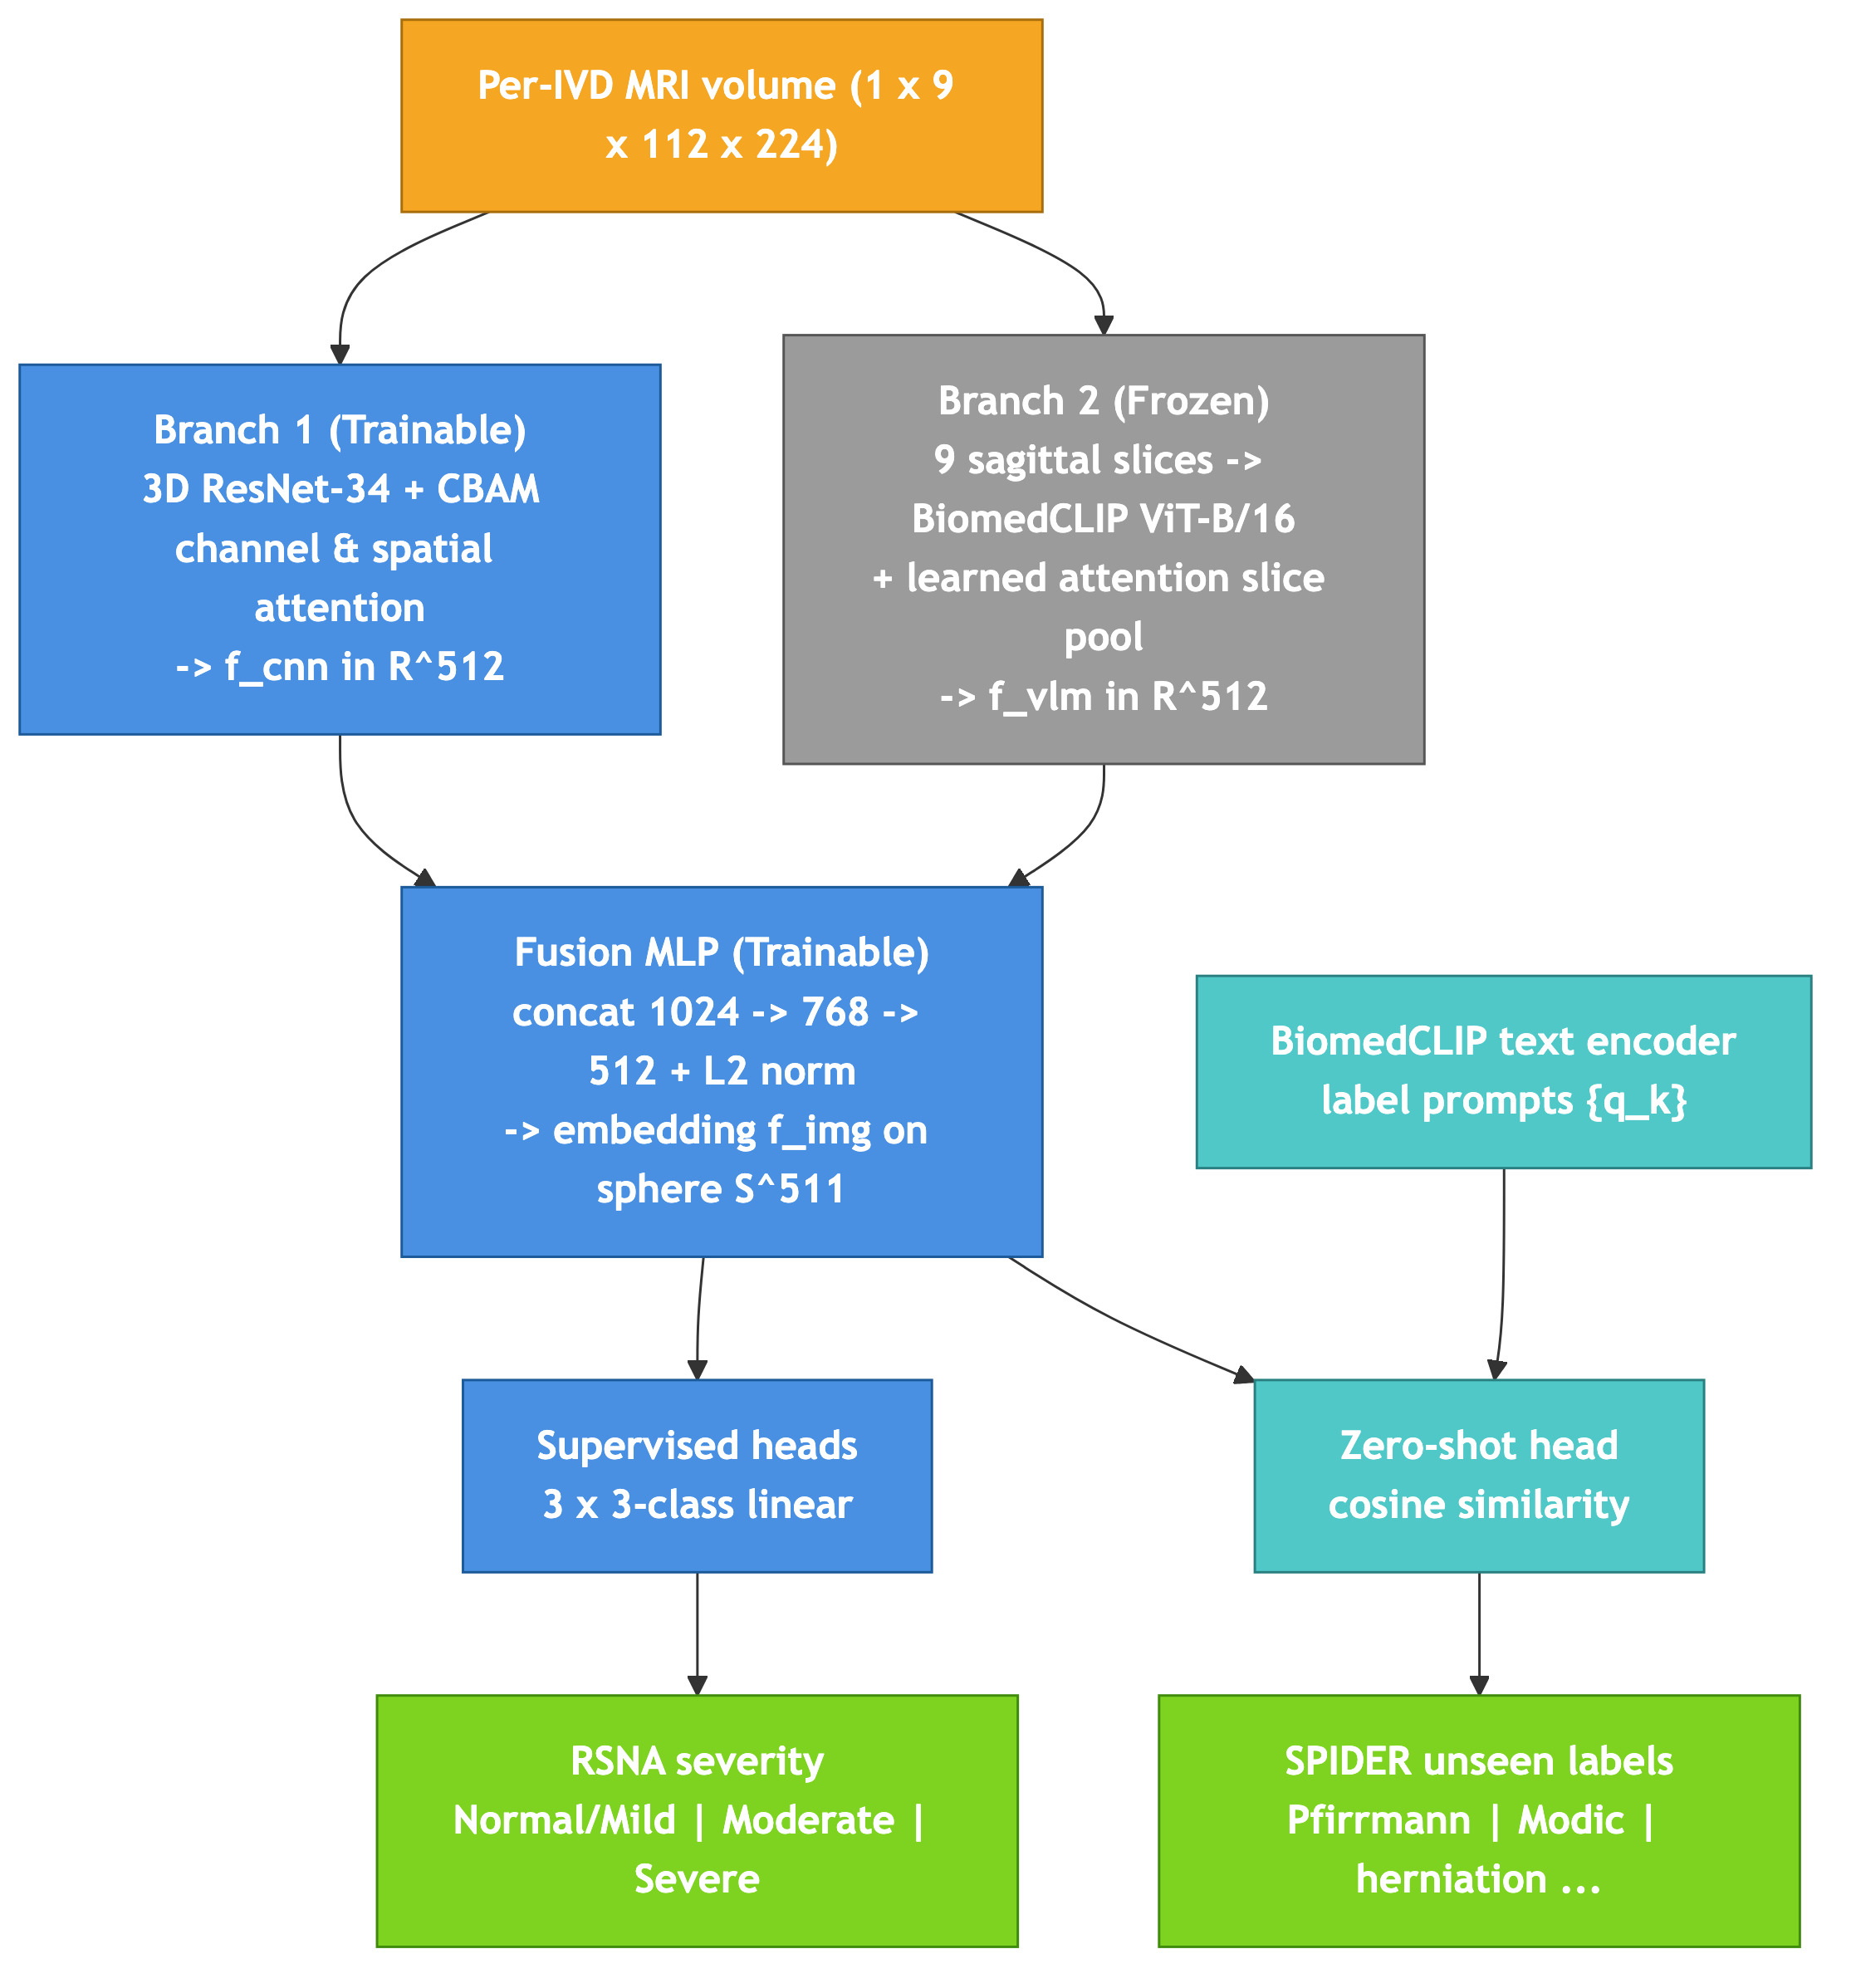
\includegraphics[width=0.52\linewidth]{hybrid_architecture_en.png}
\caption{Two-branch hybrid architecture. The fusion MLP and slice attention pool (about 1.18\,M trainable parameters) are the only learned components; the cosine-similarity head supports both supervised and zero-shot classification.}
\label{fig:arch}
\end{figure}

\subsection{Training Objective and Class-Imbalance Workflow}\label{sec:objective}

We address class imbalance with a four-part pipeline. The per-task loss is the focal cross-entropy~\cite{lin2017focal},
\begin{equation}
\mathrm{FL}_t(p_t) = -w_{c(t)}\,(1 - p_t)^{\gamma}\, \log(p_t),
\qquad \gamma = 2.0,
\label{eq:focal}
\end{equation}
where $p_t$ is the predicted probability of the ground-truth class, the factor $(1 - p_t)^{\gamma}$ down-weights easy samples, and missing labels ($-1$) are excluded via \verb|ignore_index|; the objective sums $\mathrm{FL}_t$ over the three conditions. Three further ingredients compensate for imbalance. The class weight $w_c \propto 1/\sqrt{n_c}$ (normalized to mean one over $n_c$, the count of class $c$) reduces the Severe-to-Normal gradient ratio from about $15\times$ (linear $1/n_c$) to about $4\times$, stabilizing training. \emph{Minority oversampling} (factor 3--5) at the sampler stage is complementary: it changes the chance a Severe sample enters a batch, whereas $w_c$ reweights its gradient once inside. \emph{Medical augmentation} follows SpineNetV2~\cite{windsor2022}: horizontal flip with left/right label swap, rotation $\pm 10^{\circ}$, brightness/contrast $\pm 20\%$, and Gaussian noise $\sigma = 0.05$ at probability $0.3$. We train with AdamW (lr $10^{-4}$, batch 32, weight decay $10^{-4}$) for up to 20 epochs with patience-5 early stopping.

%==============================================%
\section{Experiments and Analysis}\label{sec4}

\subsection{Environment Settings}\label{exp1}

\textbf{RSNA 2024 LumbarDISC.}~\cite{kaggle2024} About 2{,}000 patients with sagittal T2 stacks. We use a patient-level 80/20 train/validation split (\verb|random_state = 42|), which gives 1{,}942 validation IVDs from 395 patients. Labels span 5 levels $\times$ 5 conditions $\times$ 3 severities. We restrict evaluation to three of the five conditions (canal stenosis, left and right neural foraminal narrowing) for which sagittal-only input is most clinically appropriate; left and right subarticular stenosis, which are best read on axial reformats, are left to future work. The class distribution per evaluated condition averages Normal/Mild $\approx 85\%$, Moderate $\approx 10\%$, and Severe $\approx 5\%$.

\textbf{SPIDER.}~\cite{vandergraaf2024spider} About 1{,}400 IVDs from 218 patients across four Dutch hospitals (T1 and T2-FS sagittal sequences). For consistency with the RSNA-trained encoder we use the T2-FS sagittal series only. The label schema differs from RSNA: Pfirrmann grades 1--5~\cite{pfirrmann2001}, Modic changes 0--3 (4 classes)~\cite{modic1988}, spondylolisthesis, disc herniation, disc narrowing, disc bulging, and upper/lower endplate damage (all binary). SPIDER is used for cross-dataset evaluation only; no SPIDER image is seen during RSNA training.

Figure~\ref{fig:dist} reports the class distribution of both datasets: the RSNA Severe class stays under 5\%, and several SPIDER labels are similarly skewed. This imbalance is the central difficulty the training pipeline must handle.

\begin{figure}[t]
\centering
\begin{minipage}[t]{0.49\linewidth}
\centering

\includegraphics[width=\linewidth]{rsna_class_distribution_en.png}\\[1pt]
{\scriptsize (a)}
\end{minipage}\hfill
\begin{minipage}[t]{0.49\linewidth}
\centering

\includegraphics[width=\linewidth]{spider_class_distribution_en.png}\\[1pt]
{\scriptsize (b)}
\end{minipage}
\caption{Class distribution of the two datasets. (a) RSNA 2024 per-condition severity, where Normal/Mild dominates and Severe stays under 5\%. (b) SPIDER eight-label distribution, where several pathology labels are heavily skewed toward the negative class.}
\label{fig:dist}
\end{figure}

\textbf{Evaluation metrics.} We report macro-averaged Recall, Precision, F1, AUC (one-vs-rest), and AUPRC, plus per-class Severe metrics. Macro averaging over the $C = 3$ severities, $\frac{1}{C}\sum_{c}\mathrm{metric}_c$, keeps the dominant Normal/Mild class (85\% prevalence) from masking failure on the Severe class. We report AUPRC next to AUC because, on heavily imbalanced data, AUC can stay high while a model fails to rank Severe cases meaningfully; the AUPRC random baseline equals the positive-class prevalence (about 0.05 for Severe).

\textbf{Hardware and reproducibility.} All runs use a single NVIDIA RTX 4090 (Vast.ai), 16\,GB peak memory, about \$2 per hybrid run. Training/evaluation code, the three-seed checkpoints, and per-run metric logs will be released publicly upon acceptance.

\subsection{Main Ablation on RSNA 2024}\label{exp2}

Table~\ref{tab:main} reports nine metrics on the RSNA 2024 validation split (mean $\pm$ std over three seeds) for four configurations: SpineNetV2 (the plain 3D ResNet-34 grading backbone of~\cite{windsor2022}), CBAM-only (no BiomedCLIP branch), BMC-only (no CBAM branch), and the full hybrid. The hybrid wins on every metric except Mean Accuracy, which we explain below.

\begin{table}[t]
\centering
\caption{Ablation on RSNA 2024 validation (1{,}942 IVDs / 395 patients), mean $\pm$ std over 3 seeds \{42, 123, 456\}. \textbf{Bold} = best per row; Mean Accuracy is secondary under imbalance (see text).}
\label{tab:main}
\footnotesize
\setlength{\tabcolsep}{4pt}
\begin{tabular}{@{}lcccc@{}}
\toprule
Metric & SpineNetV2 & CBAM-only & BMC-only & Hybrid \\
\midrule
Mean Accuracy        & \best{81.0 $\pm$ 0.6} & 69.5 $\pm$ 1.0 & 71.2 $\pm$ 1.7 & 72.4 $\pm$ 0.3 \\
Mean F1 macro        & 0.420 $\pm$ 0.010 & 0.477 $\pm$ 0.057 & 0.482 $\pm$ 0.019 & \best{0.527 $\pm$ 0.027} \\
Mean Recall macro    & 0.412 $\pm$ 0.005 & 0.531 $\pm$ 0.068 & 0.532 $\pm$ 0.004 & \best{0.592 $\pm$ 0.026} \\
Mean Precision macro & 0.493 $\pm$ 0.028 & 0.499 $\pm$ 0.037 & 0.508 $\pm$ 0.037 & \best{0.526 $\pm$ 0.013} \\
Mean AUC macro       & 0.835 $\pm$ 0.010 & 0.803 $\pm$ 0.050 & 0.826 $\pm$ 0.015 & \best{0.838 $\pm$ 0.018} \\
Mean AUPRC macro     & 0.530 $\pm$ 0.012 & 0.498 $\pm$ 0.051 & 0.513 $\pm$ 0.030 & \best{0.533 $\pm$ 0.024} \\
\midrule
\textbf{Severe F1}    & 0.152 $\pm$ 0.008 & 0.262 $\pm$ 0.082 & 0.268 $\pm$ 0.034 & \best{0.356 $\pm$ 0.017} \\
\textbf{Severe AUC}   & 0.872 $\pm$ 0.011 & 0.865 $\pm$ 0.050 & 0.885 $\pm$ 0.010 & \best{0.899 $\pm$ 0.011} \\
\textbf{Severe AUPRC} & 0.284 $\pm$ 0.019 & 0.278 $\pm$ 0.099 & 0.275 $\pm$ 0.052 & \best{0.333 $\pm$ 0.042} \\
\bottomrule
\end{tabular}
\end{table}

\textbf{Hybrid beats either branch alone.} The hybrid F1 (0.527) exceeds both single branches (CBAM-only 0.477, BMC-only 0.482), a 4.5-point gain over the better branch that indicates the two sources are complementary rather than redundant.

\textbf{The Severe class is the headline.} Severe F1 rises 2.3$\times$ (0.152 to 0.356), Severe Recall about 4$\times$ (12.3\% to 48.6\%), and Severe AUC to 0.899; the Severe AUPRC of 0.333 against the $\approx$0.05 prevalence baseline is a 6.7$\times$ gain over chance. The 8.6-point Mean Accuracy drop is the cost of this rebalancing: SpineNetV2 scores high accuracy only by predicting Normal/Mild almost everywhere, so the hybrid trades majority-class accuracy for minority-class recall, a trade-off that is clinically reasonable at operating points where missing a Severe case costs more than a false alert.

\subsection{Cross-Dataset Zero-Shot Transfer to SPIDER}

Published work on SPIDER has focused mostly on segmentation~\cite{vandergraaf2024spider}; to our knowledge this is the first reported cross-dataset zero-shot transfer (RSNA to SPIDER) via text-prompt label-space extension. We freeze the RSNA-trained hybrid and replace the heads with cosine similarity against text prompts for the eight SPIDER categories, using no SPIDER training data. Each class uses a fixed prompt ``a magnetic resonance image of \emph{[label]}'' (e.g.\ ``lumbar disc herniation'' vs.\ ``no disc herniation''), written a priori without tuning on SPIDER, so no target-label leakage occurs. Table~\ref{tab:spider} reports per-disease zero-shot F1 over the full SPIDER cohort (1{,}439 IVDs from 208 patients): the hybrid reaches mean F1 = 0.362 across the eight unseen labels, which the SpineNetV2 and CBAM-only configurations cannot do because their fixed 3-class heads cannot accommodate a new label space without retraining.

\begin{table}[t]
\centering
\caption{Zero-shot transfer to SPIDER (no fine-tuning), recomputed from cosine predictions. \emph{OTS} = off-the-shelf BiomedCLIP (no RSNA training); \emph{Hybrid} = our RSNA-trained model. AUC = Hybrid one-vs-rest macro. \textbf{Bold} = higher F1.}
\label{tab:spider}
\begin{tabular}{@{}lccc@{}}
\toprule
SPIDER label              & OTS F1 & Hybrid F1 & Hybrid AUC \\
\midrule
Disc bulging              & 0.363 & \best{0.613} & 0.829 \\
Disc herniation           & 0.532 & \best{0.563} & 0.772 \\
Disc narrowing            & 0.403 & \best{0.586} & 0.834 \\
\midrule
Upper endplate            & \best{0.569} & 0.467 & 0.740 \\
Lower endplate            & \best{0.558} & 0.468 & 0.738 \\
Pfirrmann (5-class)       & 0.152 & \best{0.155} & 0.687 \\
Modic (4-class)           & \best{0.071} & 0.018 & 0.454 \\
Spondylolisthesis         & \best{0.500} & 0.028 & 0.807 \\
\midrule
Mean (disc-morphology)    & 0.433 & \best{0.587} & 0.812 \\
Mean (all 8)              & \best{0.394} & 0.362 & 0.733 \\
\bottomrule
\end{tabular}
\end{table}

The transfer is selective. On the three disc-morphology labels closest to the RSNA training schema (bulging, herniation, narrowing) the RSNA-trained hybrid clearly beats the off-the-shelf BiomedCLIP baseline (Table~\ref{tab:spider}), confirming the RSNA-supervised fusion adds transferable features. On labels far from that schema (endplate, spondylolisthesis) the off-the-shelf baseline is competitive or better, so its mean F1 over all eight labels (0.394) edges the hybrid (0.362): RSNA supervision helps only where the label is semantically close. Ranking and thresholding also diverge: spondylolisthesis reaches AUC 0.807 yet F1 0.03, so the embedding orders cases while the fixed cosine threshold mis-calibrates them. The Modic gap (AUC 0.45) is a task-input limit: SPIDER's fat-suppressed T2-FS lacks the paired T1 sequence Modic grading conventionally needs.

\subsection{Supervised Transfer on the SPIDER 8-Label Schema}
\label{sec:spider_transfer}

To assess transfer beyond zero-shot, we fine-tune lightweight task-specific heads (RSNA backbone frozen) on the SPIDER training split for 15 epochs, across all four configurations and the full 8-label schema (Pfirrmann 5-class, Modic 4-class, six binary labels); Table~\ref{tab:spider_transfer_agg} reports the aggregate results. The 8-label set is split 80/20 at patient level (939 training / 234 validation IVDs, 34 validation patients); backbone parameters stay frozen for a fair comparison, and only the condition-specific heads (and the fusion MLP for Hybrid and BMC-only) are trained.

\begin{table}[t]
\centering
\caption{SPIDER transfer learning, four configurations, mean across 8 conditions on validation (234 IVDs), reported as mean $\pm$ standard deviation over 3 seeds $\{42, 123, 456\}$. \textbf{Bold} = best per row (co-bolded when the top pair is statistically tied, $p>0.05$); inference is within seed noise. $^\ast$ = significant gain over CBAM (footnote).}
\label{tab:spider_transfer_agg}
\footnotesize
\begin{tabular}{@{}lcccc@{}}
\toprule
Metric & SpineNetV2 & CBAM & BMC-only & Hybrid \\
\midrule
Mean Accuracy & \best{80.23 $\pm$ 0.94} & 79.27 $\pm$ 1.19 & 76.12 $\pm$ 0.83 & 78.30 $\pm$ 1.64 \\
Mean F1 macro & \best{0.646 $\pm$ 0.002} & 0.619 $\pm$ 0.010 & 0.613 $\pm$ 0.006 & \best{0.653 $\pm$ 0.014}$^\ast$ \\
Mean AUC      & \best{0.842 $\pm$ 0.006} & 0.824 $\pm$ 0.018 & 0.808 $\pm$ 0.011 & \best{0.846 $\pm$ 0.018}$^\ast$ \\
Mean AUPRC    & \best{0.633 $\pm$ 0.026} & 0.580 $\pm$ 0.016 & 0.544 $\pm$ 0.007 & 0.611 $\pm$ 0.010 \\
\midrule
Inference (ms/sa) & 65.5 $\pm$ 2.7 & 66.7 $\pm$ 3.2 & 65.2 $\pm$ 3.9 & 66.4 $\pm$ 3.7 \\
\bottomrule
\end{tabular}

\vspace{2pt}
{\raggedright\scriptsize
$^\ast$Paired $t$-test over three seeds (per-seed Mean F1, Hybrid: 0.660/0.665/0.633, CBAM: 0.621/0.630/0.606): Hybrid vs.\ CBAM is significant ($\Delta=+0.034$, $p=0.011$, 95\% CI $[0.018,0.049]$); Hybrid vs.\ SpineNetV2 is parity ($p=0.57$).\par}
\end{table}

Two findings stand out. The hybrid and SpineNetV2 are at parity on aggregate SPIDER metrics: the F1 gap of $+0.006$ sits within seed noise and SpineNetV2 even leads slightly on AUPRC, so we do not claim the hybrid surpasses it here. The more telling result is that CBAM-only drops below plain SpineNetV2 on transfer (Mean F1 $0.619$ vs.\ $0.646$, $|\Delta|/\sigma = 3.8$), while the hybrid recovers above CBAM by $+0.034$ (paired $t$-test $p=0.011$). We analyze this asymmetry in Section~\ref{sec:disc}.

\textbf{Per-condition recovery on rare classes.}
The aggregate gains concentrate in the rare positive classes ($\leq 5\%$ prevalence). On Disc Herniation, SpineNetV2 and CBAM recall no positive case ($0\%$) while BMC-only and the hybrid recover $27.0\%$ and $35.6\%$; the BiomedCLIP prior drives most of this, with CBAM adding an incremental gain when fused. The same ordering holds for Spondylolisthesis and Pfirrmann Grade~4.

\subsection{Visualization and Discussion}\label{sec:disc}

Figure~\ref{fig:gradcam} shows Grad-CAM activation for three Severe validation cases (one per evaluated condition), comparing the CBAM-only and Hybrid branches against the final CBAM stage of the trainable branch. On the canal case the activation concentrates on the central canal narrowing rather than spreading across the whole disc, which gives qualitative support to the CBAM spatial-attention hypothesis. On the foraminal conditions Severe recall settles at 18--22\%, matching the sagittal-only literature ceiling reported by Nigru et al.~\cite{nigru2024} (balanced accuracy about 0.69--0.70); these conditions are best read on axial reformats, which we leave to future work.

\begin{figure}[t]
\centering

\includegraphics[width=0.5\linewidth]{grad_cam_severe.png}
\caption{Grad-CAM (Severe-class logit, final CBAM stage, upsampled to input resolution) for three Severe validation cases. Rows: spinal canal, left and right foraminal. Columns: input mid-sagittal slice, CBAM-only branch, full Hybrid.}
\label{fig:gradcam}
\end{figure}

\textbf{Why CBAM despite its cross-dataset cost.} CBAM both helps and hurts, depending on the setting. In-domain, both branches lift Severe F1 over SpineNetV2 to a similar degree (CBAM-only 0.262, BMC-only 0.268; Table~\ref{tab:main}), and the hybrid combines them to reach 0.356. Out-of-domain (Section~\ref{sec:spider_transfer}), CBAM falls below plain SpineNetV2 ($|\Delta|/\sigma = 3.8$), consistent with overfitting RSNA-specific patterns that do not transfer, while the hybrid recovers above CBAM ($p=0.011$) to SpineNetV2 parity. We therefore read this behavioral pattern not as an additive combination that beats SpineNetV2, but as a regularization effect that restores SpineNetV2-level transfer once CBAM is added, with BiomedCLIP serving as a reliable fallback when CBAM's in-domain bias is misaligned with the target distribution; we do not claim a mechanistic proof here. We also tested the trivial-ensemble explanation directly: averaging the SpineNetV2 and BMC-only softmax outputs reaches only Mean F1 0.45 and Severe F1 0.18 (two-seed mean), well below the learned-fusion hybrid (0.53 and 0.36), so the concat-MLP fusion is not reducible to a logit average (though the ensemble ranks slightly better on AUC/AUPRC).

\textbf{Clinical reading.} A Severe recall of 48.6\% (about 4$\times$ over baseline) is still below the $\approx$80\% sensitivity a screening tool needs, so the model is best used as a second-reader assistant that flags candidate Severe cases for radiologist confirmation rather than as a standalone tool.

\textbf{Limitations.} The regularization claim rests on a cross-dataset performance pattern (behavioral evidence); a mechanistic account through representation and domain-shift analysis is left to future work. Results use three seeds under a fixed compute budget; the small inter-seed deviations (Table~\ref{tab:main}) indicate stable estimates, but with only three seeds the reported $p$-values are exploratory rather than confirmatory. The supervised-transfer validation is small (34 patients), though the zero-shot transfer is evaluated on the full SPIDER cohort (208 patients). BiomedCLIP is frozen and 2D; native-3D MRI vision-language models were not public during this work, and the fusion is restricted to concat-MLP. Finally, RSNA Severe inter-rater agreement was not released~\cite{kaggle2024}, so the Severe ceiling reflects label noise as well as model capacity.

%==============================================%
\section{Summary}\label{sec5}

We presented a hybrid CBAM-3D and frozen-BiomedCLIP model for lumbar IVD grading on RSNA 2024. It improves Severe-class metrics (three-seed Recall $\sim$4$\times$, F1 2.3$\times$, AUC 0.899) at a controlled accuracy trade-off and extends zero-shot to eight unseen SPIDER labels. The three-seed SPIDER study shows CBAM degrading cross-dataset F1 below SpineNetV2 while frozen BiomedCLIP restores it, an effect we interpret as cross-dataset regularization. Future work includes a mechanistic representation analysis, a RadCLIP-style slice-pooling adapter~\cite{lu2024radclip}, and axial-T2 fusion.

% ----- Acknowledgments removed for double-blind review; restore for camera-ready -----
% \begin{credits}
% \subsubsection{\ackname} We acknowledge Ho Chi Minh City University of Technology (HCMUT), VNU-HCM for supporting this study.
% \subsubsection{\discintname} The authors have no competing interests to declare that are relevant to the content of this article.
% \end{credits}
%
\bibliographystyle{splncs04}
\bibliography{references}

\end{document}
